\chapter{System}
\label{sec:system}

In the following the system will be described.
Figure~\ref{fig:system} gives an overview of it.
The transmitters on the left are assumed to be widely spaced, so that they experience no coupling among each other.
The signals are transmittet over a spatial interference channel, therefore a transmitted signal reaches every receiver.
\begin{figure}[h]
\begin{center}
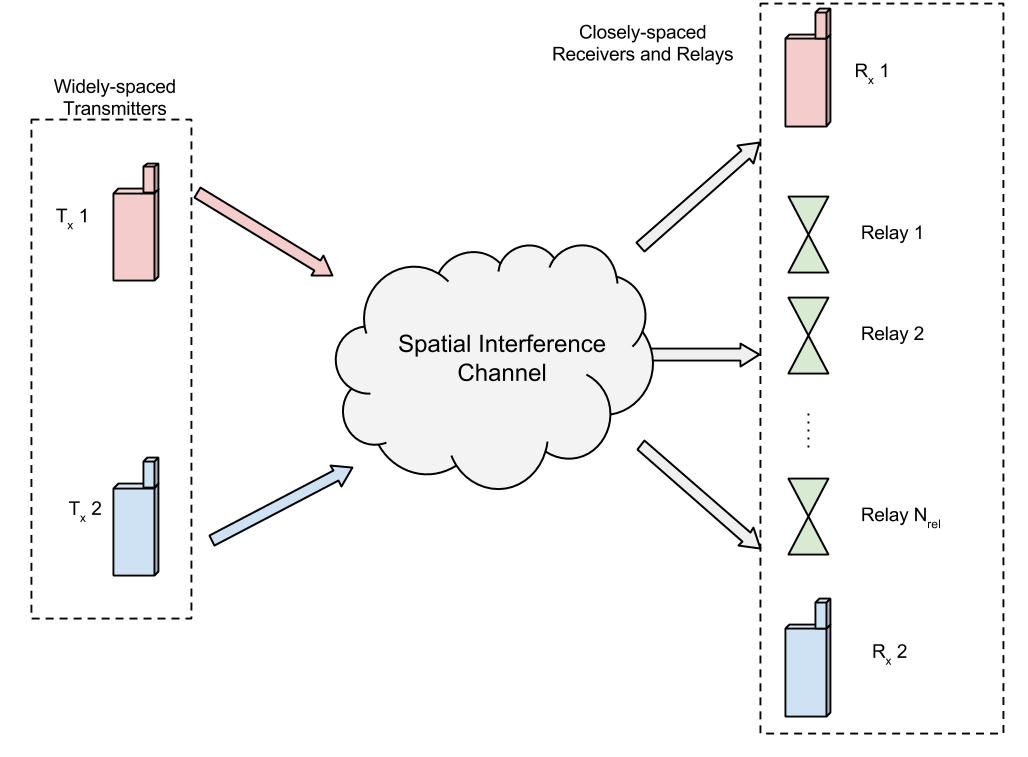
\includegraphics[width=\textwidth]{images/System.png}
\caption{Overview of the system.}
\label{fig:system}
\end{center}
\end{figure}

Besides the receivers, there are passive relays on the right side.
The relays and the receivers are closely spaced, therefore the channels between a transmitter and the receivers and relays are spatially correlated and the elements on the receiver side experience coupling among each other.

\section{Spatial Channel}
\label{sec:spatial}

TO-DO

$\mat{H}_{ij}^{\text{sp}} = $ 

\begin{figure}[h]
\begin{center}
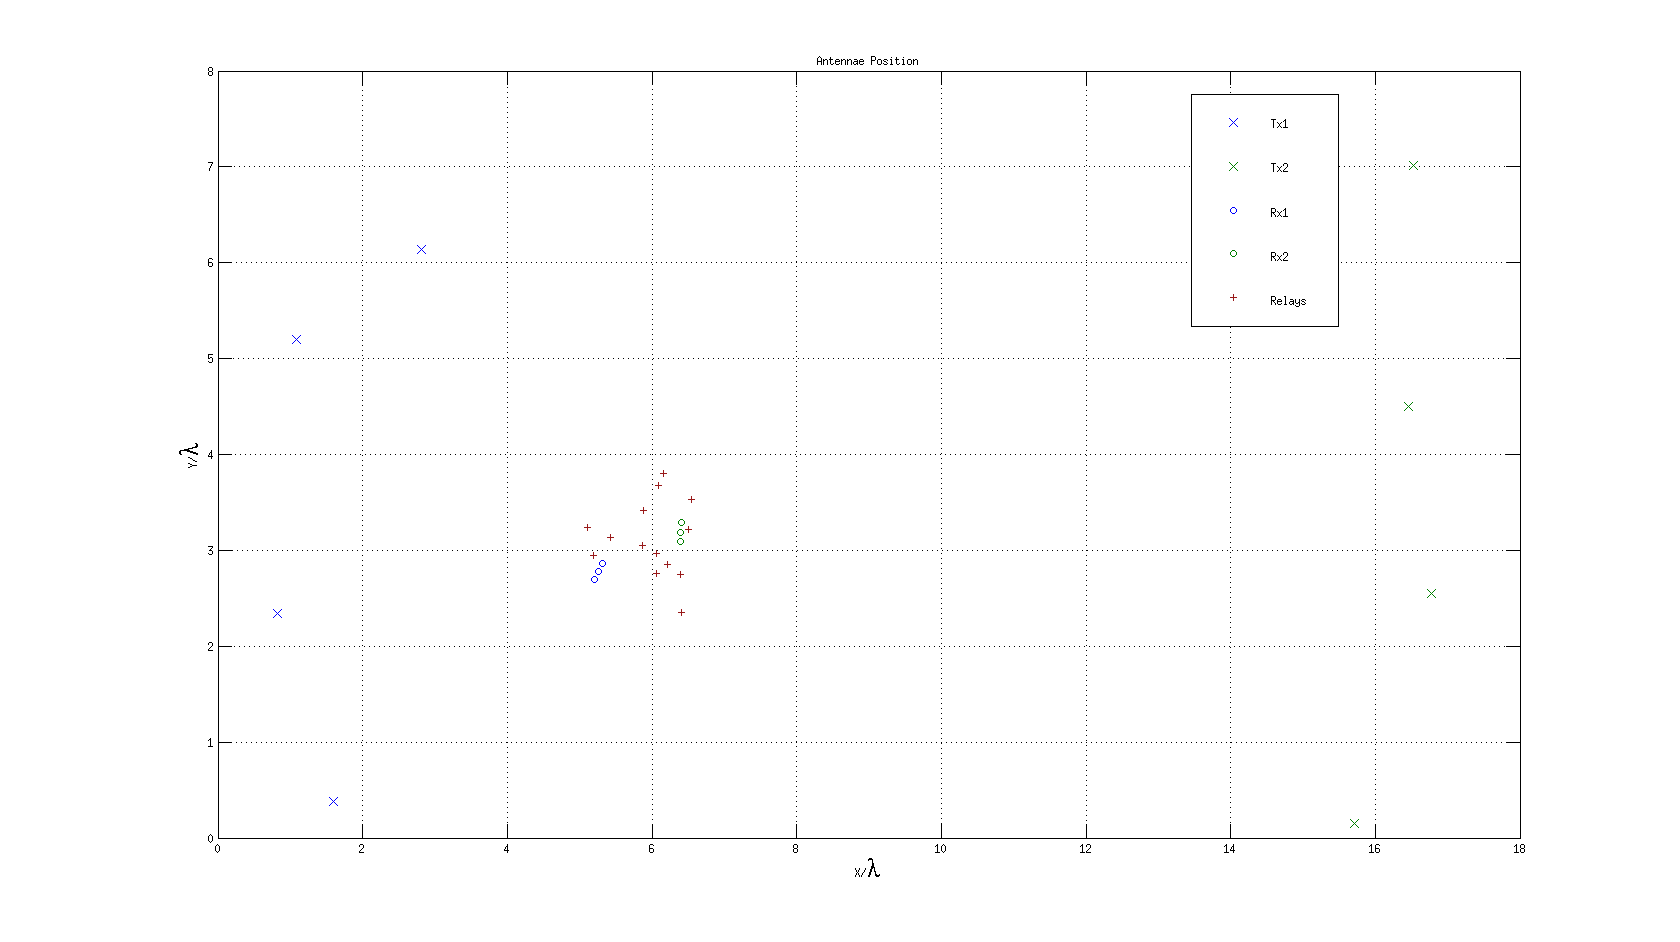
\includegraphics[width=0.75\textwidth]{images/antennae_position.png}
\caption{Example of the antenna Placing.}
\label{fig:antenna_placing}
\end{center}
\end{figure}

\section{Receiver Circuit Description}
\label{sec:network_description}
As mentioned in Section~\ref{sec:SoA}, the idea of describing the receiver circuitry is based on the work of~\cite{Nossek}.
To do so, we represent each receiver block (shown in Figure~\ref{fig:receiver}) by n-ports.
A short overview on 2-ports (simplified n-ports) is given in the following.

\subsection{Multiport Networks}
\label{sec:multiport_networks}

\begin{figure}[h]
\begin{center}
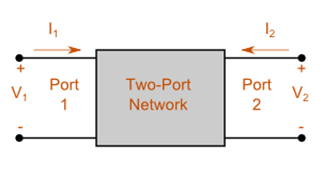
\includegraphics[width=0.75\textwidth]{images/twoport.png}
\caption{A twoport network~\cite{magnus:twoport}.}
\label{fig:twoport}
\end{center}
\end{figure}
In the following a 2-port network will be analyzed.
Later this can be easily extendet to a multiport network.

Figure~\ref{fig:twoport} shows a 2-port network.
The twoport network can be represented by its impedance matrix $\mat{Z}$.
The elements $Z_{ij}$ of the matrix are defined in the following way:
\begin{align}
\label{eq:multiport_impedance}
Z_{ij} &= \frac{V_i}{I_j},\\\nonumber
&\text{for the currents}\quad I_l = 0,\quad l\neq j.
\end{align}
Therefore the 2-port's input/output relations can be written as
\begin{align}
\label{eq:twoport_io}
\begin{bmatrix}
V_1\\V_2
\end{bmatrix} &= \mat{Z} \cdot
\begin{bmatrix}
I_1\\I_2
\end{bmatrix}
\end{align}

For a multiport network, elements $V_1,V_2,I_1\quad\text{and}\quad I_2$ become vectors, and the elements $Z_{ij},\quad i,j\in\{1,2\}$ become submatrices.
Looking from the left into the network with a load $R_L$ attached to port two, the equivalent input impedance becomes
\begin{equation}
\label{eq:eq_imp_load}
\mat{Z}_{in_1} = \mat{Z}_{11} - \mat{Z}_{21}\cdot(\mat{Z}_{22} + R_L\cdot\mat{I})^{-1}\cdot \mat{Z}_{12}.
\end{equation}
With no load attached on port two, the equivalent input impedance becomes
\begin{equation}
\label{eq:eq_imp_oc}
\mat{Z}_{in_1} = \mat{Z}_{11}.
\end{equation}
Last, having port one short-circuited and looking from port two into the network, the equivalent network impedance becomes
\begin{equation}
\label{eq:eq_imp_sc}
\mat{Z}_{in_2} = \mat{Z}_{22} - \mat{Z}_{12}\cdot(\mat{Z}_{11})^{-1}\cdot \mat{Z}_{21}.
\end{equation}
For reciprocal (multiport-)networks (\textit{RLC}-Networks, containing only passive elements), $\mat{Z}_{12} = \mat{Z}_{21}^T$.

\subsection{Receiver Blocks}
\begin{figure}[h]
\centering
  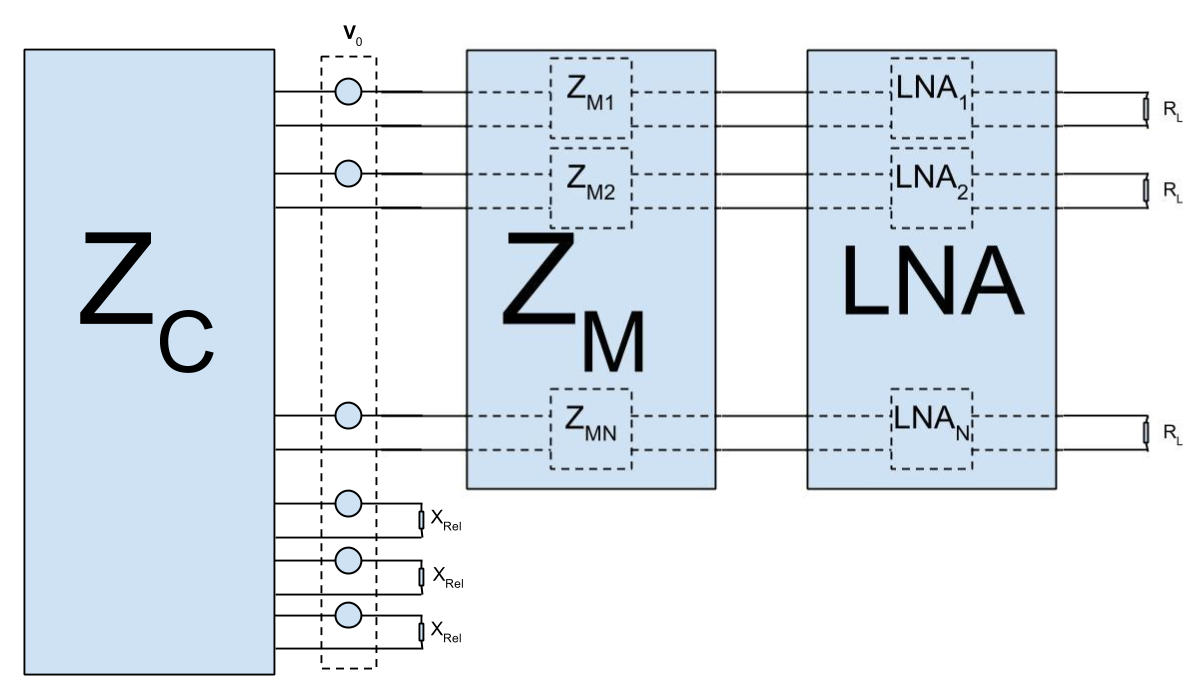
\includegraphics[width=\linewidth]{images/Receiver.png}
\caption{The receiver, with the coupling network $\mat{Z}_C$, the SP-matching network $\mat{Z}_M$, the LNA, and loads attached to the LNA.}
\label{fig:receiver}
\end{figure}
The receiver (as shown in Figure~\ref{fig:receiver}) consists of three blocks.
From left to right:
\begin{enumerate}
\item{the coupling network ($\mat{Z}_C$),}
\item{the matching network ($\mat{Z}_M$), and}
\item{the low-noise-amplifier ($\mat{LNA}$).}
\end{enumerate}
 
All these blocks can be described in multiport networks.
In the following each block will be discussed.

\subsubsection{The Coupling Network}
\label{sec:coupling_network}
The coupling network comes from the fact, that compact antenna arrays are used.
The strength of the coupling between two antennas depends on the spacing between the antennas.
In the following a unform spacing of the antennas is assumed.
As the effect of coupling from one antenna to another is the same like the reverse, the impedance matrix $\mat{Z}_C$ becomes symmetric.


\subsubsection{The Matching Network}
Behind the each receiving antenna a matching network placed, to improve the performance of the receiver.
For complexity and bandwith reasons ("WCNC - Paper"), single-port (SP) matching is assumed.
The matching network has the form of 
\begin{equation}
\mat{Z}_M=
\begin{bmatrix}
\mat{Z}_{M11} & \mat{Z}_{M12} \\
\mat{Z}_{M21} & \mat{Z}_{M22}
\end{bmatrix}.
\end{equation}
For a matching network to be lossles it must be pure imaginary and symmetric\cite{Nossek}.
Because we assume SP matching the submatrices become diagonal, with the additional property of $\mat{Z}_{M12} = \mat{Z}_{M21}^T \implies \mat{Z}_{M12} = \mat{Z}_{M21}$.


\subsubsection{The Low-Noise-Amplifier}
In the LNA-block the received signal after the matching network gets amplified.
As in the matchig network the LNA can be represented in the following way
\begin{equation}
\mat{LNA}=
\begin{bmatrix}
\mat{c} & \mat{d} \\
\mat{e} & \mat{g}
\end{bmatrix}.
\end{equation}
As each branch has it's own LNA, the submatrices $\mat{c},\mat{e}\text{ and }\mat{g}$ are again diagonal.
Additionally, matrix $\mat{d}$ is an all-zeros matrix if the unilateral assumtion (\textit{the input of the LNA is not affected by the output of the LNA}) is applied.

\subsection{Transfer Function of the Receiver}
\label{sec:transf}
The main interest lies in the transfer function of the input voltages $\vec{v}_0$ to the voltage measured at the loads (in Figure~\ref{fig:receiver}) $\vec{v}_L$.
In the following the transferfunction over each block of the receiver will be derived.
We use the termination: $\vec{v}_i$ is the voltage on the left of the block $i$ (i.e. $v_{M}$ is the voltage on the left ports of the matching network).
Additionally, we see the left ports as input ports and the right ports as output ports of each block.

For the derivation of the transferfunction we need four equivalent impedance matrices, namely
\begin{enumerate}
\item{$\mat{Z}_{eqM_1}$, the impedance matrix looking from the left into the matching network,}
\item{$\mat{Z}_{eqM_2}$, the impedance matrix looking from the right into the matching network,}
\item{$\mat{Z}_{eqLNA_1}$, the impedance matrix looking from the left into the LNA, and}
\item{$\mat{Z}_{eqLNA_2}$, the impedance matrix looking from the right into the LNA.}
\end{enumerate}

To calculate $\mat{Z}_{eqM_1}$ and $\mat{Z}_{eqLNA_1}$, we use Equation~\eqref{eq:eq_imp_load} and get the following
\begin{align}
\label{eq:zeqm1}
\mat{Z}_{eqM_1} &= \mat{Z}_{M11} - \mat{Z}_{M21}\cdot(\mat{Z}_{M22} + \mat{Z}_{eqLNA_1})^{-1}\cdot\mat{Z}_{M12},\\
\label{eq:zeqlna1}
\mat{Z}_{eqLNA_1} &= \mat{c} - \mat{e}\cdot(R_L\mat{I}_{N_r} + \mat{g})^{-1}\cdot\mat{d} = \mat{c}.
\end{align}

As we step through the receiver blocks from left to right, we always have the parallel voltages applied to each receiver block on the left.
Therefore the equivalent input impedances $\mat{Z}_{eqM_2}$ and $\mat{Z}_{eqLNA_2}$ can be derived using Equation~\eqref{eq:eq_imp_oc} and lead to the following
\begin{align}
\label{eq:zeqm2}
\mat{Z}_{eqM_2} &= \mat{Z}_{M22} - \mat{Z}_{M12}\cdot(\mat{Z}_{M11})^{-1}\cdot\mat{Z}_{M21},\\
\label{eq:zeqlna2}
\mat{Z}_{eqLNA_2} &= \mat{g} - \mat{d}\cdot(\mat{c})^{-1}\cdot\mat{e} = \mat{g}.
\end{align}

To get the parallel input voltage on the left of the matching network, we use the principle of a voltage divider as
\begin{equation}
\vec{v_M} = \mat{Z}_{eqM_1}\cdot(\mat{Z}_{eqM_1} + \mat{Z}_{C})^{-1} \cdot \vec{v_0}
\end{equation}

To transfer the voltages from the left ports to the right ports of each block we proceed for each block in the following: 
\begin{enumerate}
\item{Calculate the input currents,}
\item{transfer the input currents to the output voltages in series, and}
\item{calculate the output voltages in parallel, by a voltage divider.}
\end{enumerate}
For the matching network, it follows:
\begin{align}
\vec{i_M} &= \mat{Z}_{M11}^{-1}\cdot\vec{v_M},\\
\vec{v}_{LNA_{series}} &= \mat{Z}_{M12}\cdot\vec{i_M} = \mat{Z}_{M12} \mat{Z}_{M11}^{-1}\cdot\vec{v_M},\\
\vec{v}_{LNA} &= \mat{Z}_{eqLNA_1}(\mat{Z}_{eqLNA_1}+\mat{Z}_{eqM_2})^{-1}\cdot\vec{v}_{LNA_{series}}\\\nonumber
&=\mat{Z}_{eqLNA_1}(\mat{Z}_{eqLNA_1}+\mat{Z}_{eqM_2})^{-1}\mat{Z}_{M12} \mat{Z}_{M11}^{-1}\cdot\vec{v_M},
\end{align}
and equivalent for the LNA block
\begin{align}
\vec{v_{L}}&=R_L\mat{I}_{N_R}(R_L\mat{I}_{N_R}+\mat{Z}_{LNA_2})^{-1}\mat{Z}_{LNA12}\mat{Z}_{LNA11}^{-1}\cdot\vec{v}_{LNA}.
\end{align}
Therefore we have three transfer functions to characterize our system.
Denoting the transfer function form voltage $\vec{v}_j$ to voltage $\vec{v}_i$ as $\mat{H}_{i,j}$ (i.e. $\vec{v}_i = \mat{H}_{i,j} \cdot\vec{v}_j$), it follows
\begin{align}
\mat{H}_{M,0'} &= \mat{Z}_{eqM_1}\cdot(\mat{Z}_{eqM_1} + \mat{Z}_{C})^{-1}, \\
\mat{H}_{LNA,M} &= \mat{Z}_{eqLNA_1}(\mat{Z}_{eqLNA_1}+\mat{Z}_{eqM_2})^{-1}\mat{Z}_{M12} \mat{Z}_{M11}^{-1},\quad\text{and}\\
\mat{H}_{L,LNA} &= R_L\mat{I}_{N_R}(R_L\mat{I}_{N_R}+\mat{Z}_{eqLNA_2})^{-1}\mat{Z}_{LNA12}\mat{Z}_{LNA11}^{-1}.
\end{align}

And the overall transferfunction
\begin{align}
\mat{H}_{L,0'} &= \mat{H}_{L,LNA}\cdot\mat{H}_{LNA,M}\cdot\mat{H}_{M,0'}.
\end{align}



\subsection{Port Reduction}
\label{sec:port_reduction}

\begin{figure}
\begin{center}
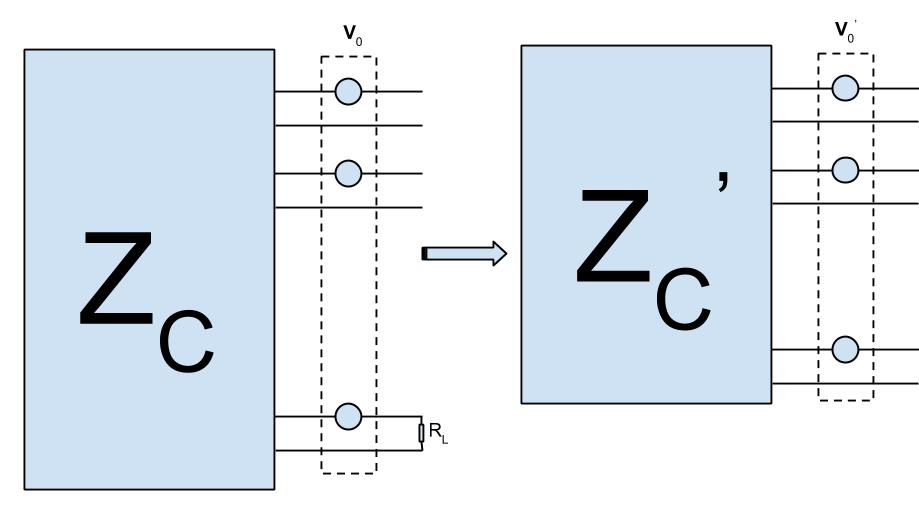
\includegraphics[width=0.75\textwidth]{images/Port_reduction.jpg}
\caption{Port reduction on a network with one load connected to the last port.}
\label{fig:port_reduction}
\end{center}
\end{figure}
In the following we describe the open circuit reduction of a system like in Figure~\ref{fig:port_reduction}.
We do the port reduction, because we are interested in the signal only at the loads of some receivers.
The signal picked up at relay antennae or not considered receivers contributes to the considered receiver by the coupling between the antennae, as described in Section~\ref{sec:coupling_network}.
Passive antennas (e.g. relay antennas) can be modeled by connecting a load directly onto the coupling network as shown in Figure~\ref{fig:port_reduction}.
Undesired receivers can be equivalently modelled, however in this case, the load corresponds to the equivalent input impedance, when looking from the left into the matching network (as in Equation~\eqref{eq:zeqm1}).
In the following, $\vec{v}_C$ denotes the voltages on the ports between the coupling matrix $\mat{Z}_C$ and the voltage sources $\vec{v}_0$, the same for the currents.
As we are not interested in the input/output-relation of these passive antennas, a port reduction is performed.
For the port reduction, the coupling matrix $\mat{Z}_C$ can be represented by four submatrices
\begin{equation}
\mat{Z}_C=
\begin{bmatrix}
\mat{Z}_{OO} & \mat{Z}_{OL}\\
\mat{Z}_{LO} & \mat{Z}_{LL}
\end{bmatrix},
\end{equation}
so that we get the system relations

\begin{align}
\label{eq:ocl_matrix}
\begin{bmatrix}
\vec{v}_{CO} \\
\vec{v}_{CL}
\end{bmatrix}
=
\begin{bmatrix}
\mat{Z}_{OO} & \mat{Z}_{OL}\\
\mat{Z}_{LO} & \mat{Z}_{LL}
\end{bmatrix}\cdot
\begin{bmatrix}
\vec{i}_{CO} \\
\vec{i}_{CL}
\end{bmatrix}.
\end{align}

The index "$O$" denotes hereby the open circuit ports, the index "$L$" the ports with a load attached.
We assume, that there are $N_R$ antennas, whereby the first $Ni$ antennas are active, and the later ones are passive (and therefore modeled by a load).
$\mat{Z}_{pass}$ denotes in the following the $N_r - N_i$ loads representing the passive antennas.
Therefore it is a diagonal matrix.

From Equation~\eqref{eq:ocl_matrix} and the property
\begin{align}
\vec{v}_{CL} &= \vec{v}_0[N_i+1:N_R]-\mat{Z}_{pass}\cdot\vec{i}_{CL}\quad\text{it follows,}\\
\vec{i}_{CL} &= -(\mat{Z}_{pass} + \mat{Z}_{LL})^{-1}\mat{Z}_{LO}\cdot\vec{i}_{CO} -\\\nonumber
&\qquad (\mat{Z}_{pass} + \mat{Z}_{LL})^{-1}\cdot\vec{v}_{0}[N_i+1:N_R]\\\nonumber\quad\text{and therefore,}&\\
\vec{v}_{CO} &= (\mat{Z}_{OO}-\mat{Z}_{OL}(\mat{Z}_{pass} + \mat{Z}_{LL})^{-1}\mat{Z}_{LO})\cdot\vec{i}_{CO} -\\\nonumber&\qquad \mat{Z}_{OL}(\mat{Z}_{pass} + \mat{Z}_{LL})^{-1}\cdot\vec{v}_0[N_i+1:N_R].
\end{align}
With this port reduction we have the new coupling matrix and the new voltage input as
\begin{align}
\mat{Z}_C^{'}&= \mat{Z}_{OO} - \mat{Z}_{OL}(\mat{Z}_{pass} + \mat{Z}_{LL})^{-1}\mat{Z}_{LO}\quad\text{and}\\
\vec{v}_0^{'} &= \mat{H}_0 \cdot \vec{v_0}\\\nonumber
&\text{with}\quad\mat{H}_0=
\begin{bmatrix}
\mat{I}_{N_i} & -\mat{Z}_{OL}(\mat{Z}_{pass} + \mat{Z}_{LL})^{-1}
\end{bmatrix},
\end{align}
and so we can reduce the system shown in Figure~\ref{fig:port_reduction}, to the system shown in Figure~\ref{fig:receiver}.

\subsection{Signal Covariance Matrix}
\label{sec:sig_cov}
To calculate the achievable sum rate of the systems, we need to derive the signal covariance matrix, defined as $\mathbb{E}[\vec{v}_L\vec{v}_L^H]$.
As in all the transfer functions from $\vec{v}_0$ to $\vec{v}_L$ only impedance matrices appear, the covariance matrix becomes
\begin{equation}
\label{eq:sig_cov}
\mat{K}_s=\mathbb{E}[\vec{v}_L^s\vec{v}_L^{s^H}] = 
	\mat{H}_{L,0}\cdot \mat{H}_{\text{sp},0} 
	\cdot\mathbb{E}[\vec{v}_0\vec{v}_0^H]\cdot
	\mat{H}_{\text{sp},0}^H \cdot \mat{H}_{L,0}^H,
\end{equation}
where $\mat{H}_{L,0}$ is the transfer function including any port reduction.

\subsection{Interference Covariance Matrix}
\label{sec:int_cov}

To calculate the interference covariance matrix, all the signal sources besides the user partner have to be consider.
In contrast to the signal covariance matrix, all signal parts arriving at the loads must be summed up over all the interferer.

The interference covariance matrix hence becomes 
\begin{equation}
\label{eq:interf_cov}
\mat{K}_i=\mathbb{E}[\vec{v}_L^i\vec{v}_L^{i^H}] = \sum_{j=1}^{N_{User}-1} 
	\mat{H}_{L,0} \cdot \mat{H}_{\text{sp},j} \cdot 
	\mathbb{E}[\vec{v}_{j}\vec{v}_{j}^H] \cdot 
	\mat{H}_{\text{sp},j}^H \cdot \mat{H}_{L,0}^H.
\end{equation}









